\documentclass[12pt,a4paper,twoside]{article}
\usepackage[latin1]{inputenc}
\usepackage{amsmath}
\usepackage{amsfonts}
\usepackage{amssymb}
\usepackage{color}
\usepackage{listings}
\usepackage{graphicx}
\usepackage{upgreek}
\usepackage{subfigure}
\usepackage{verbatim}

\author{David Hogg, Rory Holmes}
\title{Ubercalibration Simulations \\(Euclid)}
\date{Jan 2011}

\makeatletter
\def\maketitle{%
  \null
  \thispagestyle{empty}%
  \vfill
  \begin{center}\leavevmode
    \normalfont
    {\LARGE \@title\par}%
    \vskip 1cm
    {\Large \@author\par}%
    \vskip 1cm
    {\Large \@date\par}%
  \end{center}%
  \vfill
  \null
  \cleardoublepage
  }
\makeatother

\begin{document}
\maketitle

\section{Sky Catalog}
We create a fake sky, based on realistic star densities, between a magnitude of 19 to 22.5. The upper and lower limits are defined based the saturation and 10$\upsigma$ limits for a single Euclid exposure. Stars are generated with random coordinates (within the sky region being investigated) and with a random magnitude according to the following powerlaw:
\begin{equation}
\frac{1}{N} \frac{dN}{dm} = a + b m
\end{equation}

The following equation is used to generate random star magnitudes with the appropriate probability density distribution function (see Appendix for derivation):

\begin{equation}
m = \frac{1}{b} \log{(\left[ 10^{b m_{max}} - 10^{b m_{min}} \right] r + 10^{b m_{min}})}
\end{equation}

\noindent{}where r is a random number in the range [0.0, 1.0). See Fig. \ref{fig:catalog}. 

\begin{figure}[ht]
\centering
\subfigure[A histogram of the generated stars' magnitudes.]{
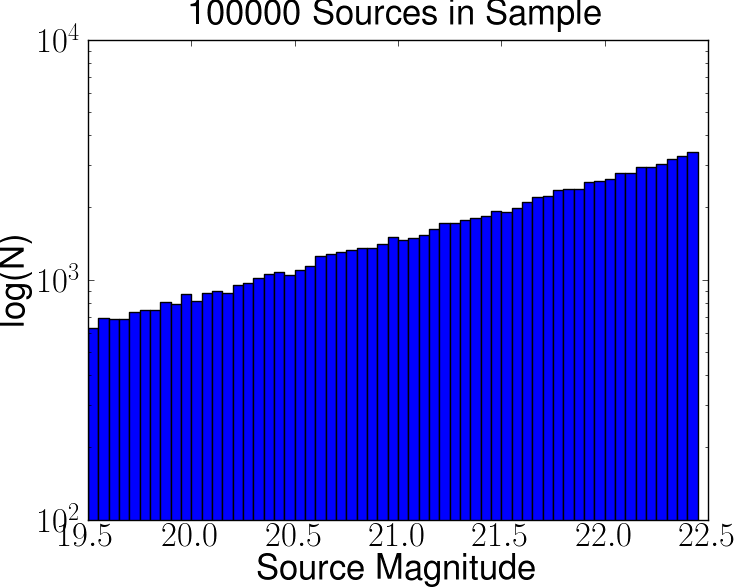
\includegraphics[width=0.45\textwidth]{source_mag_histogram.png}
\label{fig:source_magnitude}
}
\subfigure[A small subset of the simulated stars in the fake sky.]{
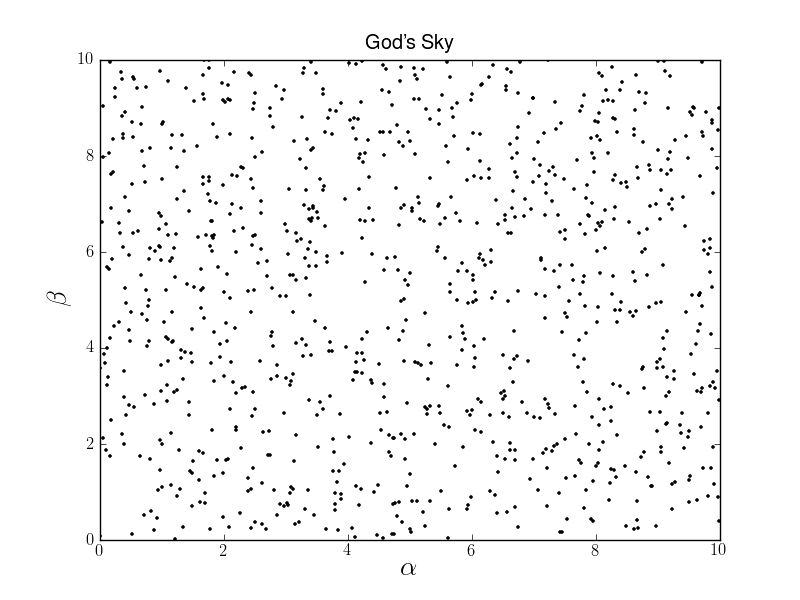
\includegraphics[width=0.45\textwidth]{gods_sky.png}
\label{fig:gods_sky}
}
\label{fig:catalog}
\end{figure}

The random number generator is given the same seed, so that the same simulated sky is produced each time the simulation is run.

\section{Single Exposure}
With a given pointing and orientation, we transform the sky catalog into focal plane coordinates and find all the stars falling within the instrument's field-of-view. The default field-of-view size is the same as the Euclid NISP instrument's. We do not simulate images, instead we trivially convert the actual star fluxes into measured fluxes. 

\subsection{Uncertainty Variance}
We assume that the Euclid exposures will be background limited and that we will hit an upper limit on the signal-to-noise for bright sources. We model the uncertainty on the flux as:

\begin{equation}
\sigma_{\text{f}}^{2} = \alpha^{2} + \eta^{2} f^{2} 
\end{equation}

\noindent{}where $\alpha$ and $\eta$ are both constants (see Fig. \ref{fig:flux_uncertainty}).

\begin{figure}[ht]
\begin{center}
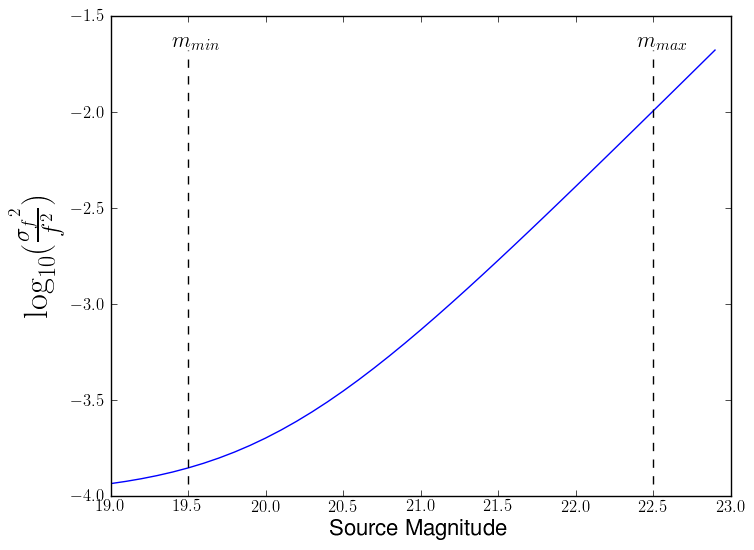
\includegraphics[width=\textwidth]{flux_uncertainty_variance.png}
\end{center}
\caption{The flux uncertainty used as a function of star magnitude.\label{fig:flux_uncertainty}}
\end{figure}

\subsection{Catalog to Measured Flux Conversion}
The measured flux from a star depends on its focal plane position ($\vec{x_i}$), God's flat-field (with parameters $\vec{q}$) and the star's true flux ($s$). 

\begin{equation}
c_i = f(\vec{x_i} | \vec{q}) . s_{k} + e_{i}
\end{equation}

\noindent{}An error, drawn from the Normal Distribution $e_{ij} = N(e|0,{\sigma_i}^2)$, is also introduced to the measurement.

\begin{figure}[ht]
\begin{center}
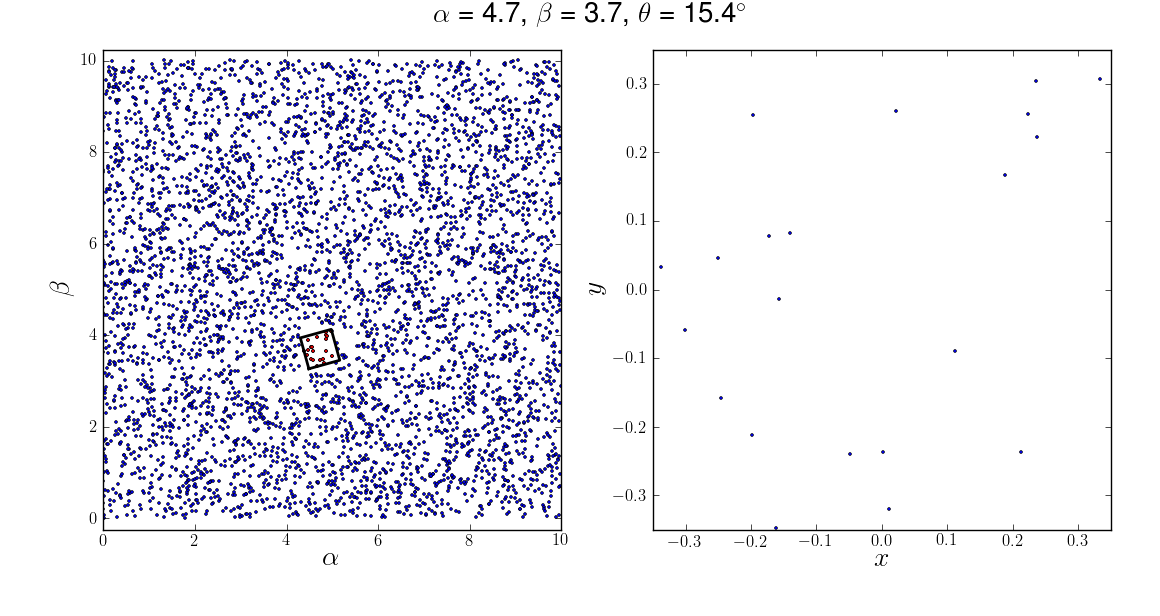
\includegraphics[width=\textwidth]{camera.png}
\end{center}
\caption{A single exposure of the sky with the pointing coordinates and the field orientation given in the title. Left: Plot of the entire fake sky, with the instrument's field-of-view shown in black and the measured sources highlighted in red. Right: The distribution of the highlighted sources on the instrument's focal plane. \label{fig:camera}}
\end{figure}


\section{Ubercalibration}
The ubercalibration procedure works in two sub-steps: (i) the star fluxes are refined based on the latest flat-field estimate (\textit{s\_step}) and (ii) the flat-field parameters are refined based on the latest star flux estimates (\textit{q\_step}). We iterate these steps until the parameters converge. In our notation $j$ refers to the iteration step. 

Our flat-field is defined by a set of parameters $\vec{q}$. After the $j$th iteration, the flat-field parameters will be indexed as $\vec{q_j}$. The individual star measurements are defined as $c_i$ (``counts''), where each $i$ corresponds to a exposure number $n$, a specific star with ID number $k$ and a focal plane position $\vec{x}$.

Our model is

\begin{equation}
c_i = f(\vec{x_i} | \vec{q_j}) . s_{kj} + e_{ij}
\end{equation}

where $s_k$ is the true flux from star $k$ and our error is drawn from the Normal Distribution $e_{ij} = N(e|0,{\sigma_i}^2)$.

\subsection{Star Flux Refinement: \textbf{\textit{s\_step}}}
The flux estimates, $s_k$, for each star can be considered individually. At step $j$ we can refine a star's flux estimate (to $s_{kj+1}$) by minimizing the error function with the latest flat-field parameters:

\begin{equation}
\chi^2_{k} = \sum_{i \in \mathcal{O}(k)} \frac{(c_i-f_{ij}s_{kj})^2}{{\sigma_i}^2}
\end{equation}

\begin{equation}
\frac{d\chi^2_{k}}{d s_{kj}} = \sum_{i \in \mathcal{O}(k)} \frac{-2 f_{ij} (c_i-f_{ij}s_{kj+1})}{{\sigma_i}^2} = 0
\end{equation}

\begin{equation}
\Rightarrow \sum_{i \in \mathcal{O}(k)} \frac{f_{ij} c_i}{{\sigma_i}^2}= \sum_{i \in \mathcal{O}(k)} \frac{f_{ij}^2 s_{kj+1}}{{\sigma_i}^2}
\end{equation}

\begin{equation}
\Rightarrow s_{kj+1} = {\sum_{i \in \mathcal{O}(k)} \frac{f_{ij} c_i}{{\sigma_i}^2}}/{\sum_{i \in \mathcal{O}(k)} \frac{f_{ij}^2}{{\sigma_i}^2}} \label{eqn:s_step}
\end{equation}

The standard uncertainty inverse variance on $s_{kj+1}$ is given by the denominator in Eqn \ref{eqn:s_step}.

\subsection{Flat-Field Refinement: \textbf{\textit{p\_step}}}
The flat-field parameters can now be refined with the latest star flux estimates. To do this we minimize the error function for all measurements with respect to the flat-field parameters.

\begin{equation}
\chi^2 = \sum_{i} \frac{(c_i-f_{ij}s_{kj+1})^2}{{\sigma_i}^2}
\end{equation}

\begin{equation}
f_{ij} = \sum_{l = 1}^L q_{lj} g_l(\vec{x_i})
\end{equation}

\begin{equation}
\chi^2 = \sum_{i} \frac{(c_i- s_{kj+1} \sum_{l = 1}^L q_{lj} g_l(\vec{x_i}))^2}{{\sigma_i}^2}
\end{equation}

\begin{equation}
\frac{d\chi^2}{dq_{lj}} = \sum_{i} \frac{-2 g_l(\vec{x_i}) s_{kj+1} (c_i- s_{kj+1} \sum_{l' = 1}^{L'} q_{l'j} g_{l'}(\vec{x_i}))}{{\sigma_i}^2} = 0
\end{equation}

\begin{equation}
\sum_{i} \frac{g_l(\vec{x_i}) s_{kj+1} c_i}{{\sigma_i}^2} = \sum_{i} \frac{g_l(\vec{x_i}) s_{kj+1}^2 \sum_{l' = 1}^{L'} q_{l'j+1} g_{l'}(\vec{x_i})}{{\sigma_i}^2}
\end{equation}

\section{Initial Results}
\subsection{Surveys}
To test the code we considered two extreme survey examples. The first, called Survey A, consists of a regular grid of pointings over the sky with a 2.5\% overlap between neighboring fields. Nine passes are performed over the sky and each time the grids are aligned exactly. The second survey, Survey D, has the same number of fields as Survey A, but the pointing and orientation of these fields are random. These two surveys can be seen in Fig. \ref{fig:surveys}.

\begin{figure}[ht]
\centering
\subfigure{
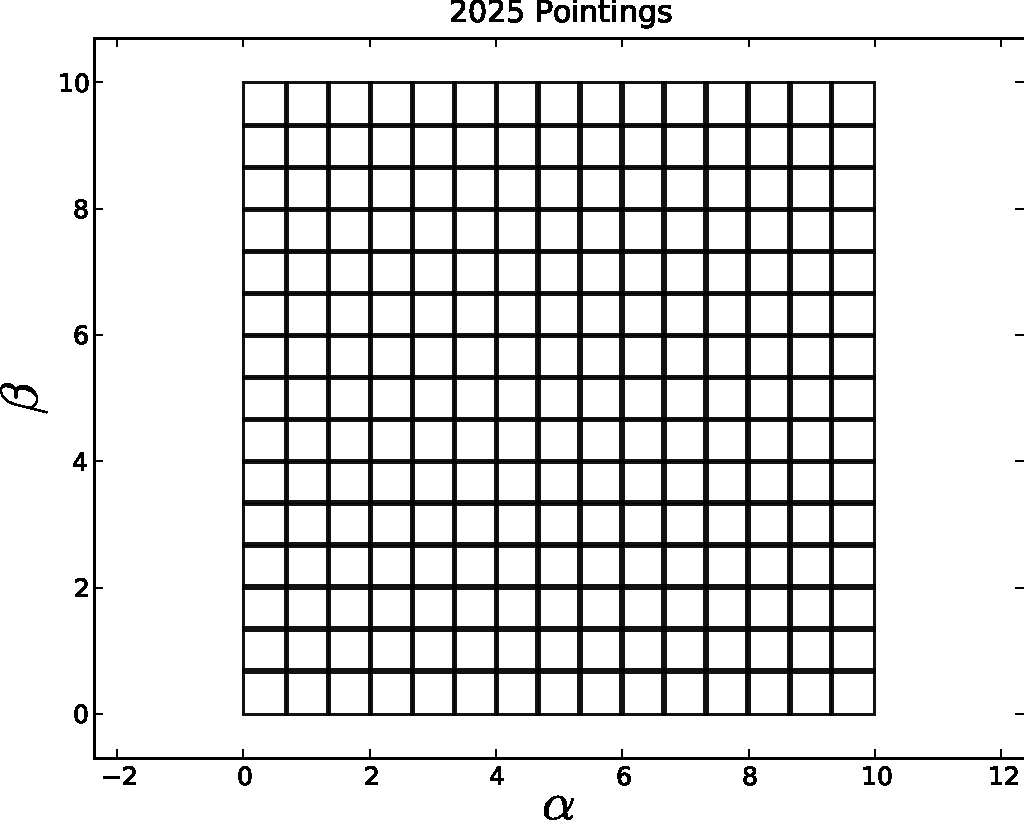
\includegraphics[width=0.47\textwidth]{A.pdf}
}
\subfigure{
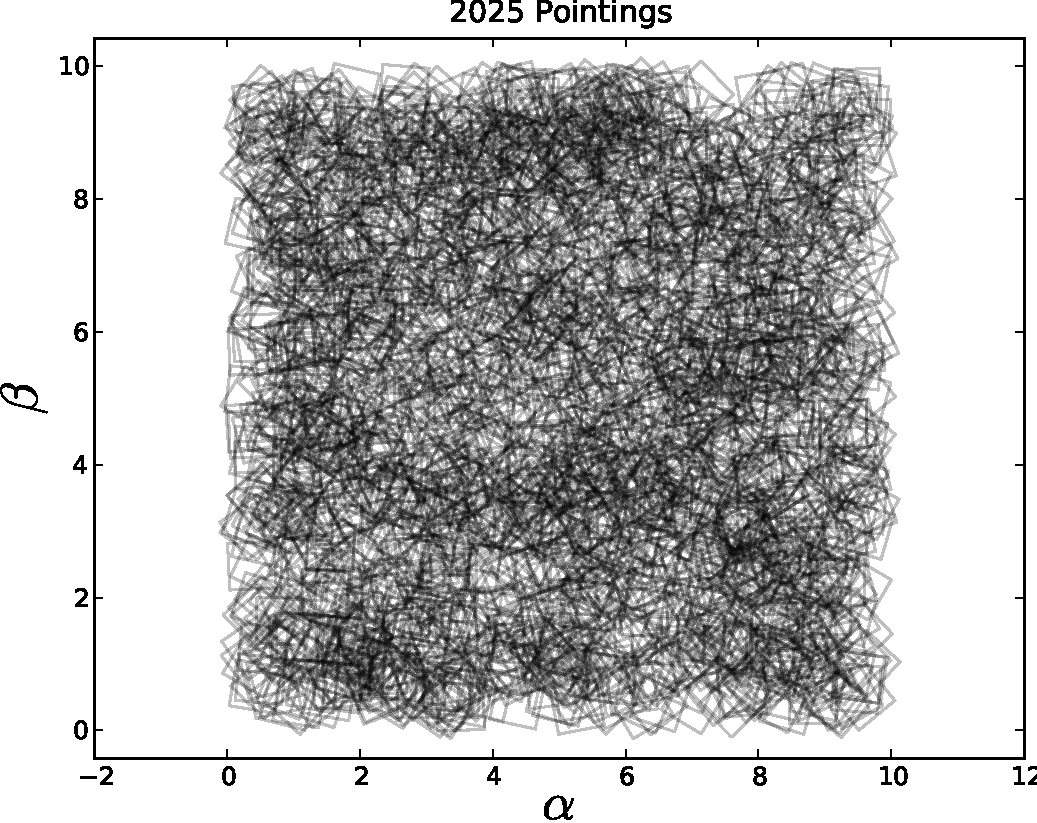
\includegraphics[width=0.47\textwidth]{D.pdf}
}
\caption{Left: The A Survey has regular pointings over the sky with a 2.5\% overlap between adjacent fields. Nine passes are performed over the sky and each time the grids are aligned exactly. Right: The D Survey has the same number of pointings as the A Survey, but the pointings and orientations are random.\label{fig:surveys}}
\end{figure}

\subsection{Ubercalibration Performance}

The difference in ubercalibration method's ability to fit the flat field and the star magnitudes for the two different surveys is striking. With the random survey (D) we can get very close to the actual flat field in a small number of ubercalibration iterations (see Fig \ref{fig:D}). The well ordered survey (A), on the other hand, does not converge to the correct flat field even with 1,000 ubercal iterations. Even when we start with almost the correct flat-field parameters (those found with the D survey - shown in Fig. \ref{fig:D}), the ubercalibration procedure does not converge. In fact, with each iteration solution drifts away from the actual flat-field. Fig \ref{fig:A} shows the fitted flat-field from Survey A after 1,000 with the initial parameters shown in Fig \ref{fig:D}.

\begin{figure}[ht]
\begin{center}
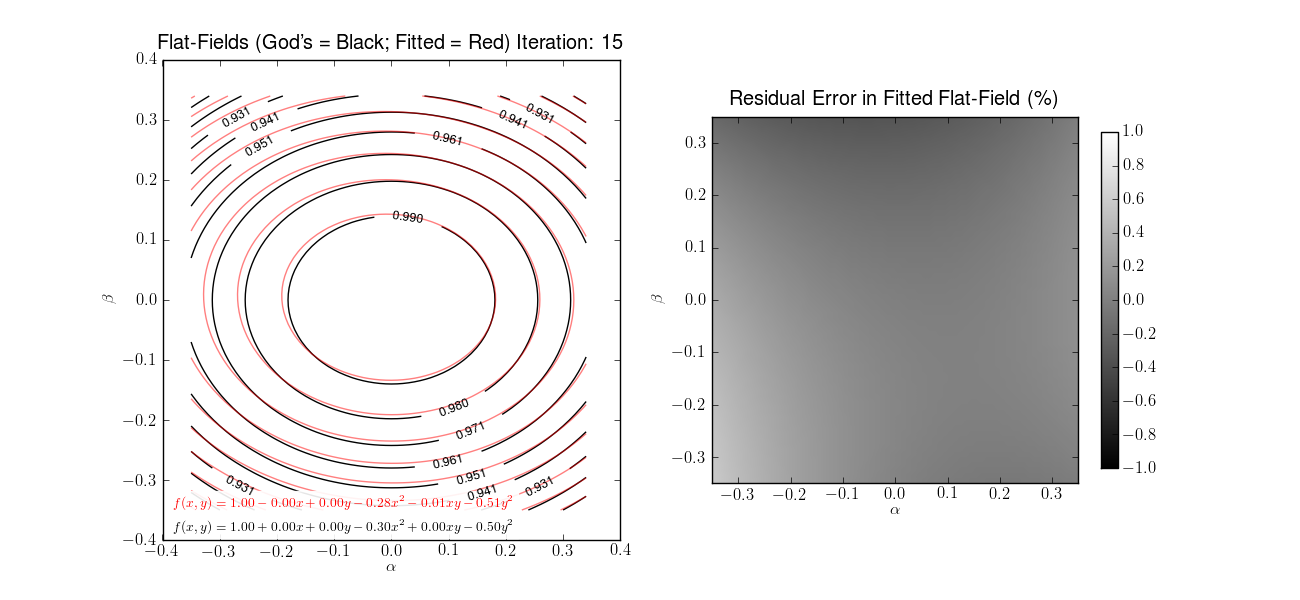
\includegraphics[width=\textwidth]{D_15_ff.png}
\end{center}
\caption{The fitted flat field compared to the actual flat field found with Survey D. \label{fig:D}}
\end{figure}

\begin{figure}[ht]
\begin{center}
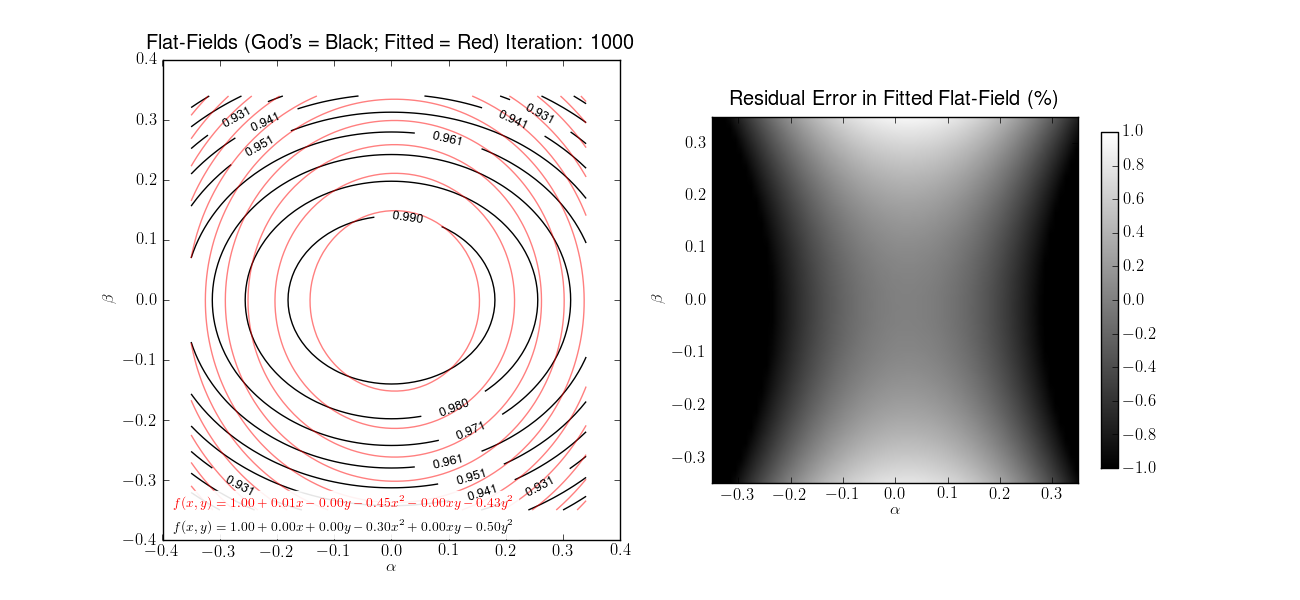
\includegraphics[width=\textwidth]{A_1000_ff.png}
\end{center}
\caption{The fitted flat field compared to the actual flat field calculated found with Survey A. The ubercalibration procedure was started with almost exact flat field parameters (those found from Survey D - see Fig. \ref{fig:D}) and has drifted away from the actual solution. \label{fig:A}}
\end{figure}

\appendix
\begin{comment}
\section{Random Magnitude Generation}
XX DAVID: I have included this so that I remember how the formula was derived...


\noindent{}The Transformation Method is used generate random numbers with the appropriate probability density function. 

\begin{equation}
\frac{1}{N} \frac{dN}{dm} = a + b m
\end{equation}

\noindent{}The probability a star is generated with a magnitude $m$ in the range [$m_0$,$m_1$) is therefore:

\begin{equation}
p(m) = \frac{\dfrac{d N}{d m}}{\int_{m_{0}}^{m_{1}}\dfrac{d N}{d m} dm} = A \frac{d N}{d m}
\end{equation}

\noindent{}Using the Transformation Method, we find:

\begin{eqnarray}
r (m) & = & \int_{m_{0}}^{m} p(m') dm'\\
& = & A \int_{m_{0}}^{m} 10^{a+b m'} dm'\\
& = & B \int_{m_{0}}^{m} e^{b m' \ln{10}} dm'\\
& = & \frac{B}{b \ln{10}} \left[ 10^{b m} - 10^{b m_{0}} \right] \label{eqn:Bover}
\end{eqnarray}

\noindent{}Since the probability of generating a magnitude between $m_0$ and $m_1$ is 1:

\begin{equation}
B = \frac{b \ln{10}}{\left[ 10^{b m_{1}} - 10^{b m_{0}} \right]} \label{eqn:B}
\end{equation}

\noindent{}Substituting Eqn. \ref{eqn:B} into Eqn. \ref{eqn:Bover} and rearranging we find that stars can be produced according to the appropriate probability density distribution function with the equation:

\begin{equation}
m = \frac{1}{b} \log{(\left[ 10^{b m_{max}} - 10^{b m_{min}} \right] r + 10^{b m_{min}})}
\end{equation}
\noindent{}where r is a random number in the range [0.0, 1.0).
\end{comment}
\end{document}
